
\section{Explored but Ineffective Approaches}
\label{sec:ineffective_approaches}

During development, we investigated several alternative strategies that, while promising in theory, did not yield satisfactory results in practice. We summarize these negative results here both for completeness and to highlight potential pitfalls for future work.  

\paragraph{Alternative CAM Generation Methods.} 
We experimented with LayerCAM and Grad-CAM++, as replacements for our primary CAM extraction mechanism. Although these methods are widely used in weakly supervised settings, in our framework they couldn't produce better CAMs. \\
LayerCAM, which uses the element-wise product of feature maps and gradients, produced better CAMs than Grad-CAM in case of single class images, shown in \autoref{fig:cam_variation_singleclass}. However, in multi-class scenarios, it almost always highlighted only one dominant region for every class, which is quite interesting. This problem is shown in \autoref{fig:cam_multiclass_a}, \autoref{fig:cam_multiclass_c} and \autoref{fig:cam_multiclass_d}. \\
Grad-CAM++ weights gradients based on their positive influence. It often missed easier classes, such as the \textit{Dog} class shown in \autoref{fig:cam_multiclass_d}. It also failed to localize the \textit{Person} class in multi-class images, as shown in \autoref{fig:cam_multiclass_b} and \autoref{fig:cam_multiclass_c}. Overall, Grad-CAM++ produced more fragmented and less false positives compared to Grad-CAM.\\
Overall, Grad-CAM provided the most consistent and complete CAMs across both single and multi-class images, making it the most suitable choice for our framework. \autoref{fig:cam_variation_multiclass_all} shows the comparison of all three methods on multiple multi-class images.

\begin{figure}[!t]
  \centering
  \setlength{\tabcolsep}{1pt}
  \renewcommand{\arraystretch}{0.7}
  \fbox{%
    \begin{minipage}{0.9\textwidth}
      %%%%%%%%%%%%% Subfigure A %%%%%%%%%%%%%
      \begin{subfigure}[t]{0.48\textwidth}
        \centering
        \begin{tabular}{c c c}
          {\scriptsize \textbf{Grad-CAM}} & {\scriptsize \textbf{Layer-CAM}} & {\scriptsize \textbf{Grad-CAM++}} \\[2pt]
          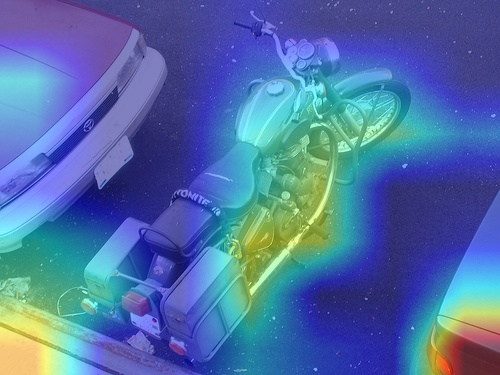
\includegraphics[width=0.32\linewidth, height=0.32\linewidth]{figures/cams/gradcam/2008_007558_6} &
          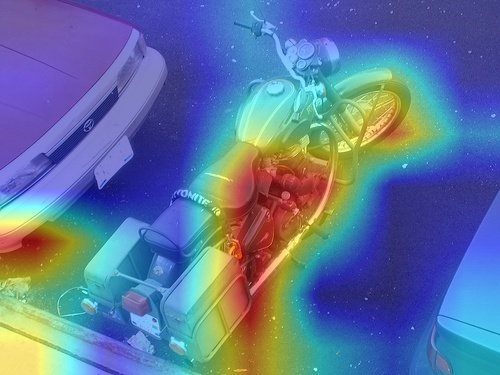
\includegraphics[width=0.32\linewidth, height=0.32\linewidth]{figures/cams/layercam/2008_007558_6} &
          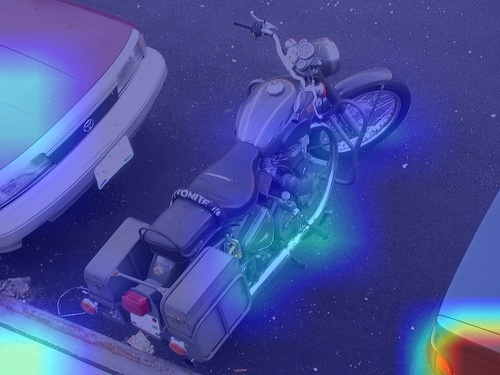
\includegraphics[width=0.32\linewidth, height=0.32\linewidth]{figures/cams/gradcampp/2008_007558_6} \\
          \multicolumn{3}{c}{{\scriptsize \textit{Class: Car}}} \\[2pt]
          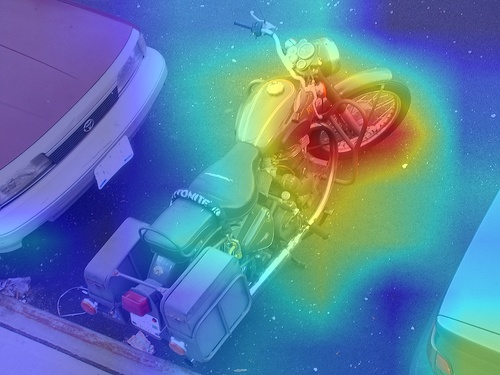
\includegraphics[width=0.32\linewidth, height=0.32\linewidth]{figures/cams/gradcam/2008_007558_13} &
          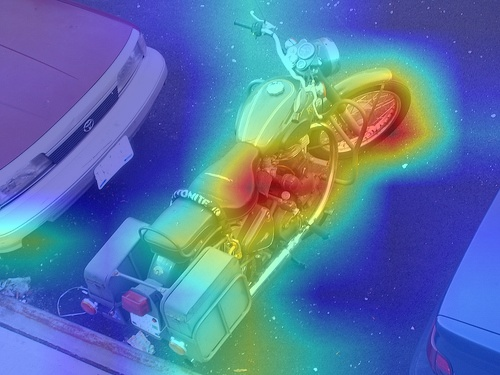
\includegraphics[width=0.32\linewidth, height=0.32\linewidth]{figures/cams/layercam/2008_007558_13} &
          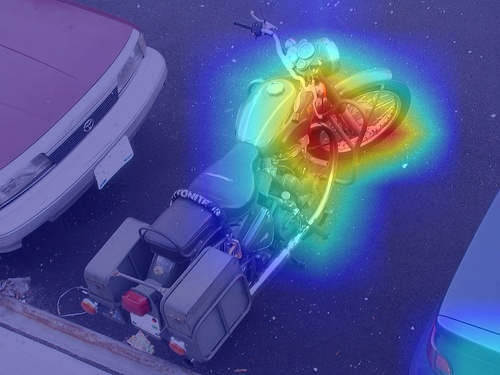
\includegraphics[width=0.32\linewidth, height=0.32\linewidth]{figures/cams/gradcampp/2008_007558_13} \\
          \multicolumn{3}{c}{{\scriptsize \textit{Class: Motorbike}}} \\
        \end{tabular}
        \caption{Example 1: Multi-class image containing \textit{Car} and \textit{Motorbike}.}
        \label{fig:cam_multiclass_a}
      \end{subfigure}
      \hfill
      %%%%%%%%%%%%% Subfigure B %%%%%%%%%%%%%
      \begin{subfigure}[t]{0.48\textwidth}
        \centering
        \begin{tabular}{c c c}
          {\scriptsize \textbf{Grad-CAM}} & {\scriptsize \textbf{Layer-CAM}} & {\scriptsize \textbf{Grad-CAM++}} \\[2pt]
          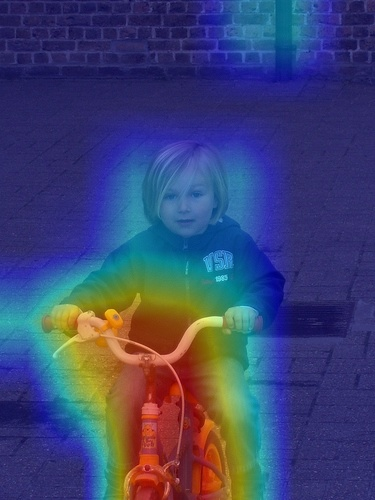
\includegraphics[width=0.32\linewidth, height=0.32\linewidth]{figures/cams/gradcam/2009_001718_1} &
          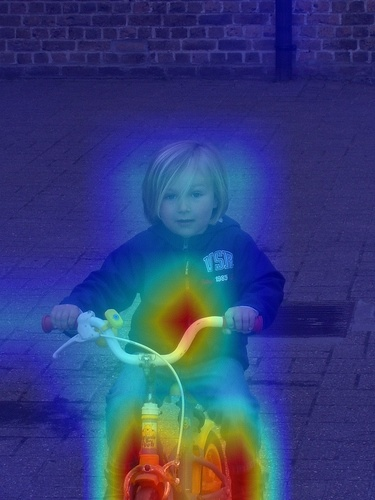
\includegraphics[width=0.32\linewidth, height=0.32\linewidth]{figures/cams/layercam/2009_001718_1} &
          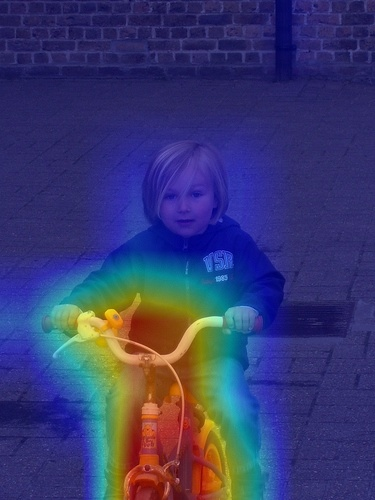
\includegraphics[width=0.32\linewidth, height=0.32\linewidth]{figures/cams/gradcampp/2009_001718_1} \\
          \multicolumn{3}{c}{{\scriptsize \textit{Class: Bicycle}}} \\[2pt]
          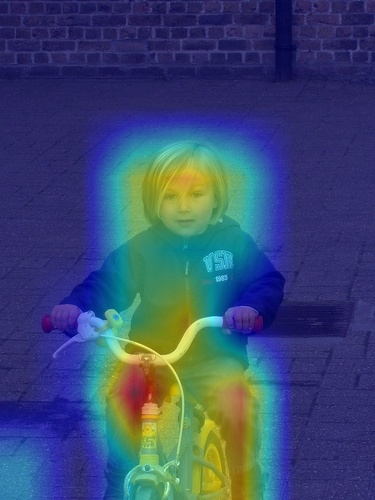
\includegraphics[width=0.32\linewidth, height=0.32\linewidth]{figures/cams/gradcam/2009_001718_14} &
          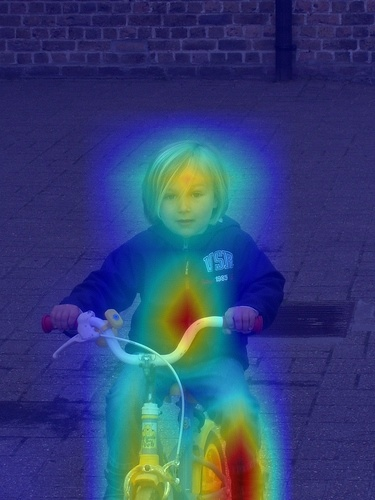
\includegraphics[width=0.32\linewidth, height=0.32\linewidth]{figures/cams/layercam/2009_001718_14} &
          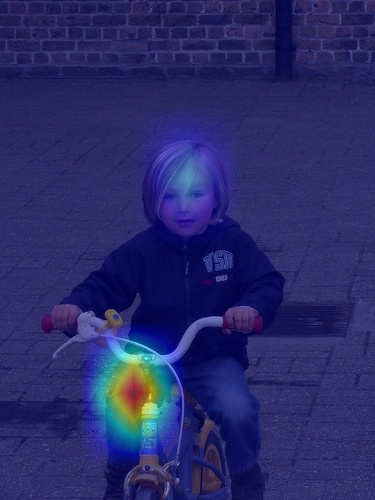
\includegraphics[width=0.32\linewidth, height=0.32\linewidth]{figures/cams/gradcampp/2009_001718_14} \\
          \multicolumn{3}{c}{{\scriptsize \textit{Class: Person}}} \\
        \end{tabular}
        \caption{Example 2: Multi-class image containing \textit{Bicycle} and \textit{Person}.}
        \label{fig:cam_multiclass_b}
      \end{subfigure}

      \vspace{8pt}

      %%%%%%%%%%%%% Subfigure C %%%%%%%%%%%%%
      \begin{subfigure}[t]{0.48\textwidth}
        \centering
        \begin{tabular}{c c c}
          {\scriptsize \textbf{Grad-CAM}} & {\scriptsize \textbf{Layer-CAM}} & {\scriptsize \textbf{Grad-CAM++}} \\[2pt]
          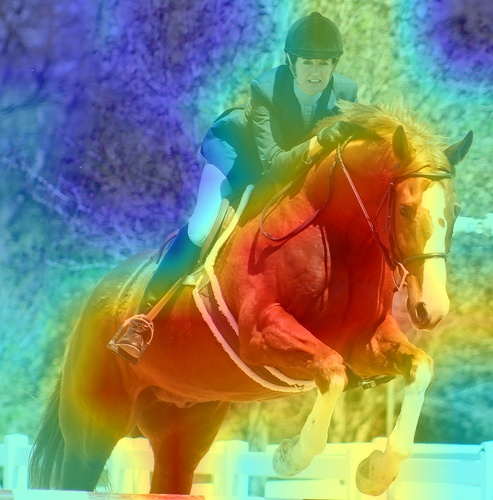
\includegraphics[width=0.32\linewidth, height=0.32\linewidth]{figures/cams/gradcam/2008_002762_12} &
          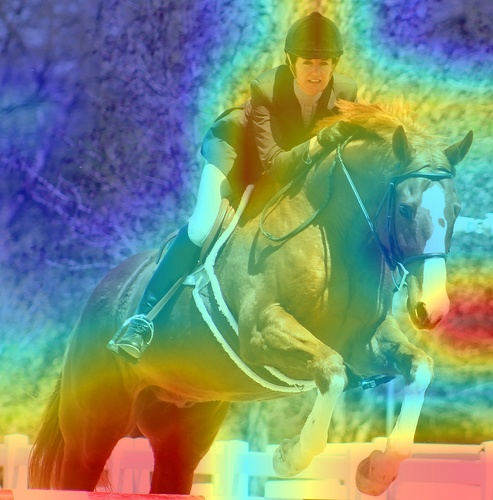
\includegraphics[width=0.32\linewidth, height=0.32\linewidth]{figures/cams/layercam/2008_002762_12} &
          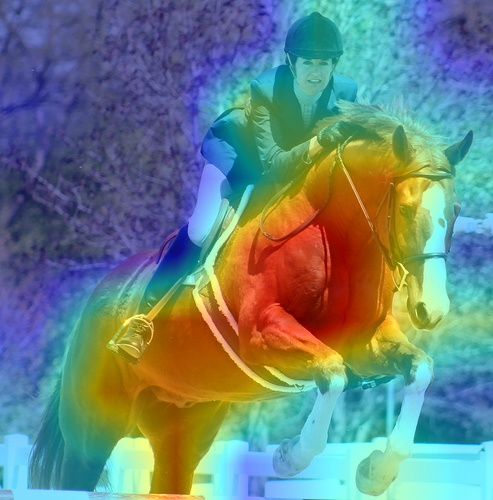
\includegraphics[width=0.32\linewidth, height=0.32\linewidth]{figures/cams/gradcampp/2008_002762_12} \\
          \multicolumn{3}{c}{{\scriptsize \textit{Class: Horse}}} \\[2pt]
          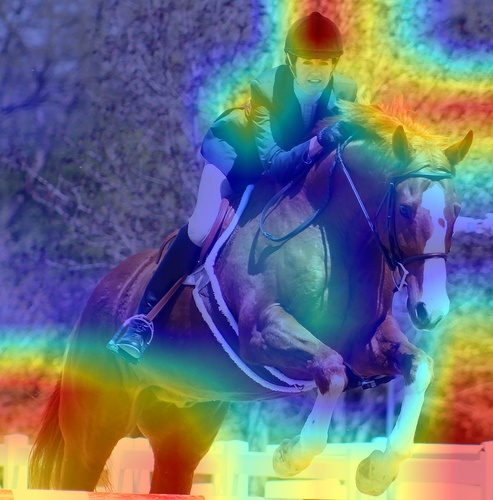
\includegraphics[width=0.32\linewidth, height=0.32\linewidth]{figures/cams/gradcam/2008_002762_14} &
          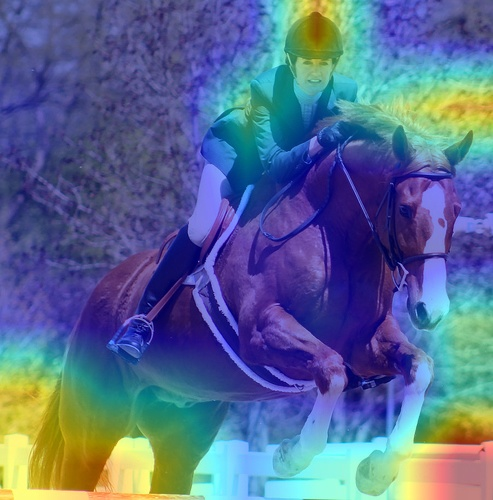
\includegraphics[width=0.32\linewidth, height=0.32\linewidth]{figures/cams/layercam/2008_002762_14} &
          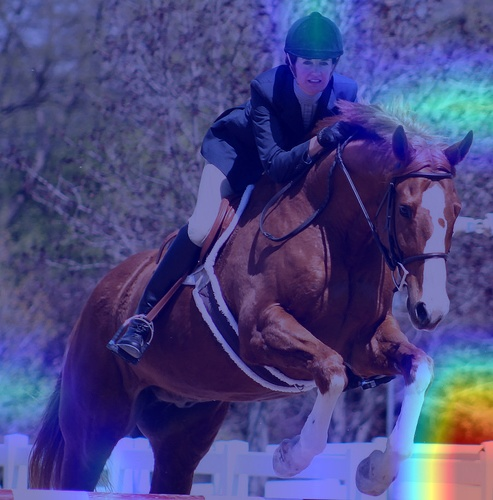
\includegraphics[width=0.32\linewidth, height=0.32\linewidth]{figures/cams/gradcampp/2008_002762_14} \\
          \multicolumn{3}{c}{{\scriptsize \textit{Class: Person}}} \\
        \end{tabular}
        \caption{Example 3: Multi-class image containing \textit{Horse} and \textit{Person}.}
        \label{fig:cam_multiclass_c}
      \end{subfigure}
      \hfill
      %%%%%%%%%%%%% Subfigure D %%%%%%%%%%%%%
      \begin{subfigure}[t]{0.48\textwidth}
        \centering
        \begin{tabular}{c c c}
          {\scriptsize \textbf{Grad-CAM}} & {\scriptsize \textbf{Layer-CAM}} & {\scriptsize \textbf{Grad-CAM++}} \\[2pt]
          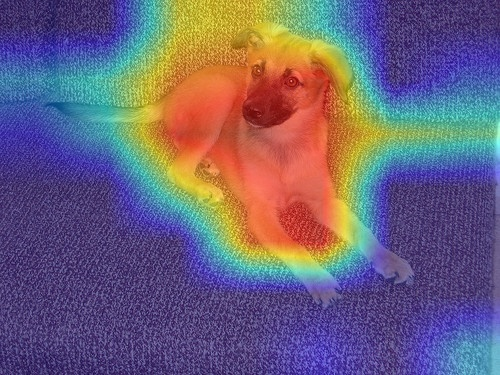
\includegraphics[width=0.32\linewidth, height=0.32\linewidth]{figures/cams/gradcam/2010_001933_11} &
          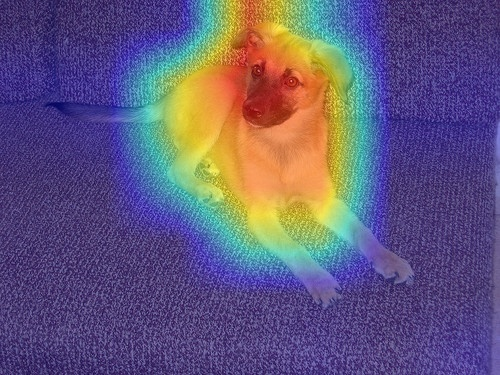
\includegraphics[width=0.32\linewidth, height=0.32\linewidth]{figures/cams/layercam/2010_001933_11} &
          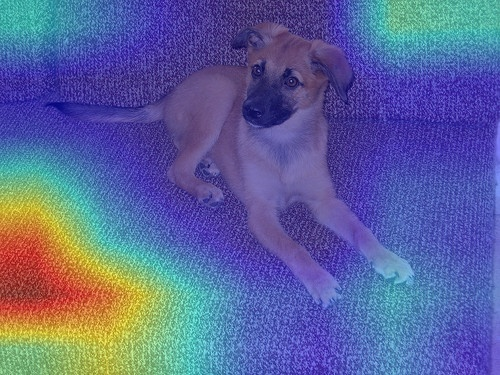
\includegraphics[width=0.32\linewidth, height=0.32\linewidth]{figures/cams/gradcampp/2010_001933_11} \\
          \multicolumn{3}{c}{{\scriptsize \textit{Class: Dog}}} \\[2pt]
          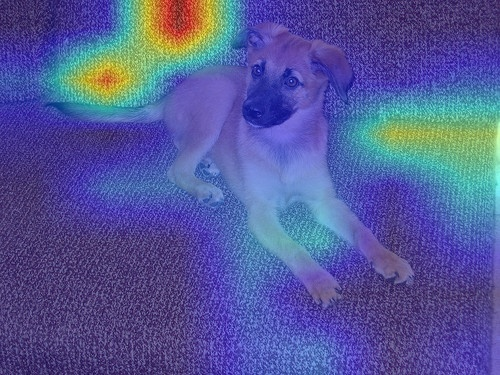
\includegraphics[width=0.32\linewidth, height=0.32\linewidth]{figures/cams/gradcam/2010_001933_17} &
          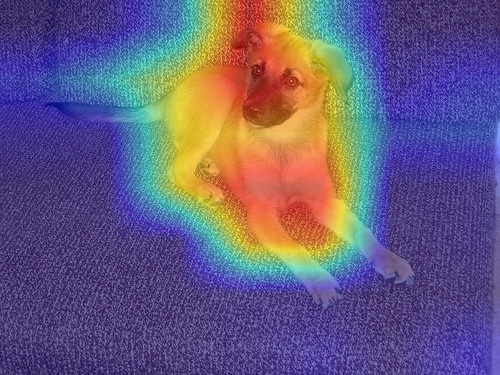
\includegraphics[width=0.32\linewidth, height=0.32\linewidth]{figures/cams/layercam/2010_001933_17} &
          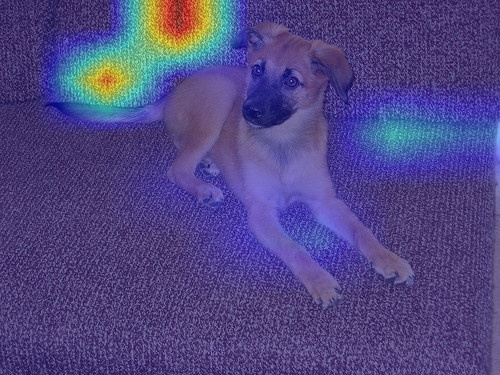
\includegraphics[width=0.32\linewidth, height=0.32\linewidth]{figures/cams/gradcampp/2010_001933_17} \\
          \multicolumn{3}{c}{{\scriptsize \textit{Class: Sofa}}} \\
        \end{tabular}
        \caption{Example 4: Multi-class image containing \textit{Dog} and \textit{Sofa}.}
        \label{fig:cam_multiclass_d}
      \end{subfigure}

      \caption{Comparison of Grad-CAM, Layer-CAM, and Grad-CAM++ visualizations for multiple multi-class images from the Pascal VOC dataset. Each subfigure shows CAMs for two distinct object classes within the same image.}
      \label{fig:cam_variation_multiclass_all}
    \end{minipage}
  }
\end{figure}



\paragraph{Backbone Fine-tuning Variants.}
We also attempted to fine-tune the last one or two Swin Transformer blocks, both with and without an additional fully connected (FC) projection layer. These modifications degraded the quality of the generated CAMs, often resulting in unstable or inconsistent activations. This suggests that partial fine-tuning, without carefully designed regularization, may overfit to local patterns and disrupt the alignment with text embeddings.  

\paragraph{Local-to-Global Attention Conversion.}
Finally, we explored replacing Swin's window-based local attention with a global attention mechanism to improve long-range reasoning. However, this approach led to a sparse and ineffective global attention matrix, which in turn degraded segmentation quality. This outcome underscores the difficulty of naively extending Swin to global attention without appropriate architectural adaptations.  

In summary, although these explorations did not improve performance, they provide valuable insights. They demonstrate the limitations of directly adopting generic CAM methods, highlight the fragility of partial backbone fine-tuning, and reveal the challenges of balancing local and global attention in window-based Transformers.
